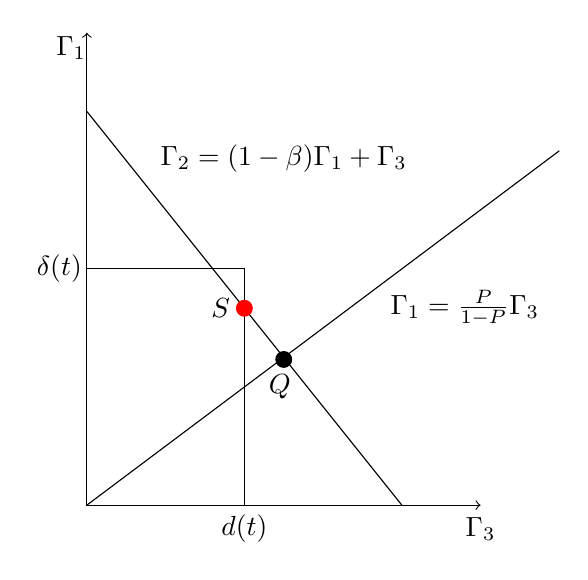
\begin{tikzpicture}
	\draw[<->] (0,6) -- (0,0) --(5,0);
	\draw (0,0) rectangle (2,3);
	\draw (4,0) -- (0,5);
	\draw (0,0) -- (4,3) -- (6,4.5);
	\draw[fill=black](2.5,1.85) circle (0.1);
	\draw[color=red, fill=red](2,2.5) circle (0.1);
	\node (below) at (5,-0.3) {$\Gamma_3$};
	\node (below) at (2,-0.3) {$d(t)$};
	\node (left) at (-0.2,5.8) {$\Gamma_1$};
	\node (left) at (-0.35,3) {$\delta(t)$};
	\node (right) at (2.5,4.4) {$\Gamma_2=(1-\beta)\Gamma_1 +\Gamma_3$};
	\node (right) at (4.8,2.5) {$\Gamma_1=\frac{P}{1-P}\Gamma_3$};
	\node (below) at (2.45,1.5) {$Q$};
	\node (left) at (1.7,2.5) {$S$};
\end{tikzpicture}